\vspace{-10mm}
\begin{IEEEbiography}[{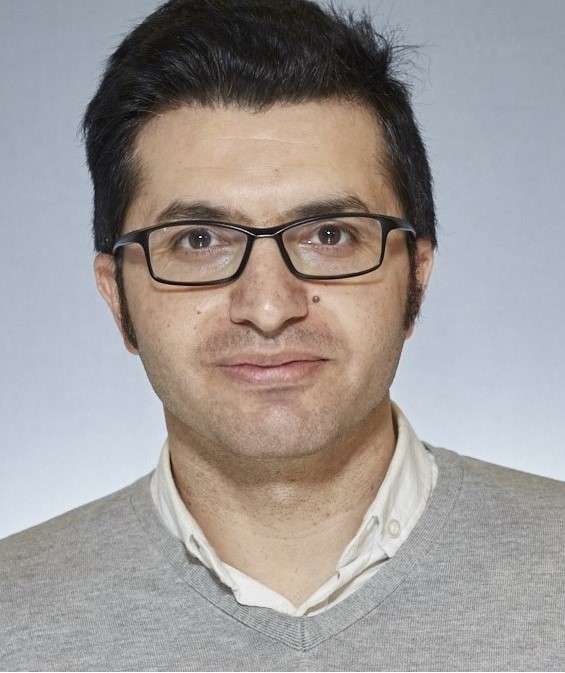
\includegraphics[width=1in,height=1.25in,clip,keepaspectratio]{alinia.png}}]{Bahram Alinia} is an R\&D software engineer in France since 2018. He received a joint PhD degree from Institute Telecom SudParis/Paris-Sorbonne University (UPMC) in 2018, a M.Sc. degree of IT engineering from university of Tehran, Iran,  in 2012, and a B.Sc. degree of computer science from University of Tabriz, Tabriz, Iran in 2008.
%and a masters degree in Information Technology Engineering from University of Tehran, Tehran, Iran. He was a Researcher with the School of Computer Science, Institute for Research in Fundamental Sciences, Iran, from 2009 to 2012. He received a Ph.D. degree in service architecture lab, Institute Telecom SudParis, France and participated in several European projects in the domain of smart grids. His research area includes wireless communications, energy systems, transportation electrification, algorithm design and approximation.
\end{IEEEbiography}
%\vspace{-30mm}
\begin{IEEEbiography}[{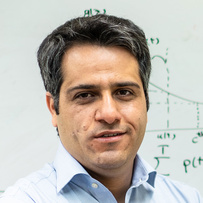
\includegraphics[width=1in,height=1.25in,clip,keepaspectratio]{hajiesmaili.png}}]{Mohammad H. Hajiesmaili} is a Research Assistant Professor in the College of Information and Computer Sciences at the University of Massachusetts Amherst. Before joining UMass, Mohammad was a postdoctoral fellow with the Johns Hopkins University, from 2017 to 2018, and with the Chinese University of Hong Kong, from 2015 to 2016. He received his Ph.D. and M.Sc. degrees from the University of Tehran, and his B.Sc. degree from Sharif University of Technology.
\end{IEEEbiography}
\begin{IEEEbiography}[{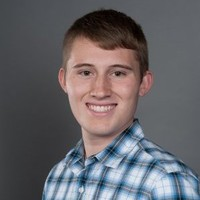
\includegraphics[width=1in,height=1.25in,clip,keepaspectratio]{lee.png}}]{Zachary J. Lee} is a Ph.D. student in Electrical Engineering at the California Institute of Technology (Caltech). He received his M.S.  in Electrical Engineering from Caltech in 2018 and his B.S.Eng. in Electrical Engineering from John Brown University in 2016. He is a recipient of the National Science Foundation Graduate Research Fellowship and Resnick Sustainability Institute Graduate Fellowship. His research is centered on smart electric vehicle charging, where he draws on broad interests in data science, computer science, and energy.
\end{IEEEbiography}
%\vspace{-30mm}
\begin{IEEEbiography}[{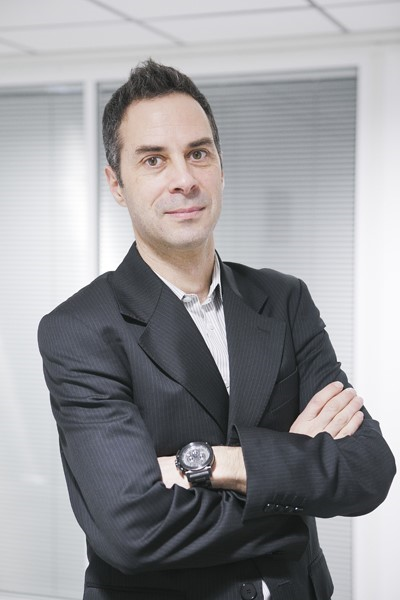
\includegraphics[width=1in,height=1.25in,clip,keepaspectratio]{crespi.png}}]{Prof. No\"{e}l Crespi} holds Masters degrees from the Universities of Orsay (Paris 11) and Kent (UK), a diplome d'ing\'{e}nieur from Telecom ParisTech, a Ph.D and an Habilitation from UPMC (Paris-Sorbonne University). From 1993 he worked at CLIP, Bouygues Telecom and then at Orange Labs in 1995. He took leading roles in the creation of new services with the successful conception and launch of Orange prepaid service, and in standardisation (from rapporteurship of IN standard to coordination of all mobile standards activities for Orange). In 1999, he joined Nortel Networks as telephony program manager, architecting core network products for EMEA region. He joined Institut Mines-Telecom in 2002 and is currently professor and Program Director, leading the Service Architecture Lab. He coordinates the standardisation activities for Institut Mines-Telecom at ITU-T and ETSI. He is also an adjunct professor at KAIST (South Korea), an affiliate professor at Concordia University (Canada), and gest researcher at the University of Goettingen (Germany). He is the scientific director the French-Korean laboratory ILLUMINE. His current research interests are in Data Analytics, Internet of Things and Softwarisation.
http://noelcrespi.wp.tem-tsp.eu/
\end{IEEEbiography}	
\begin{IEEEbiography}[{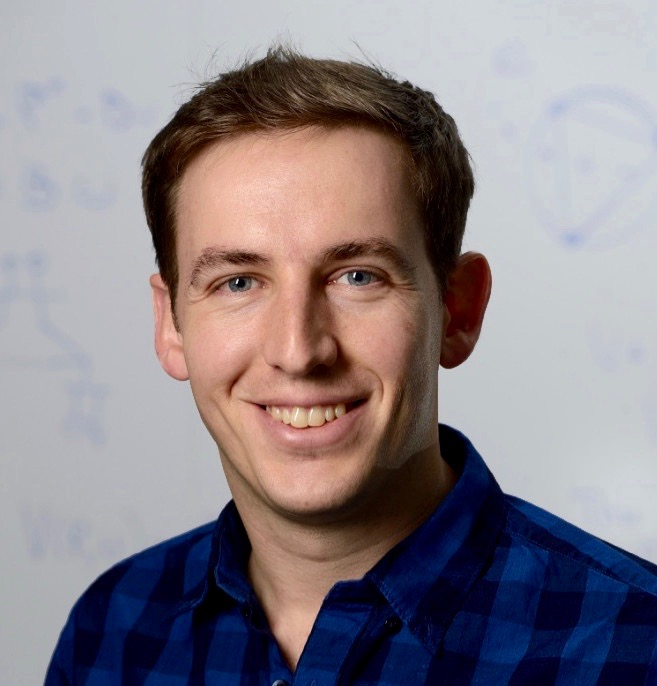
\includegraphics[width=1in,height=1.25in,clip,keepaspectratio]{mallada.png}}]{Enrique Mallada} is an assistant professor of electrical and computer engineering at Johns Hopkins University since 2016. Before joining Hopkins, he was a post-doctoral fellow at the Center for the Mathematics of Information at the California Institute of Technology from 2014 to 2016. He received his ingeniero en telecomunicaciones (telecommunications engineering) degree from Universidad ORT, Uruguay, in 2005 and his Ph.D. degree in electrical and computer engineering with a minor in applied mathematics from Cornell University in 2014. Dr. Mallada was awarded the NSF CAREER award in 2018, the ECE Director's Ph.D. Thesis Research Award for his dissertation in 2014, the Cornell University's Jacobs Fellowship in 2011 and the Organization of American States scholarship from 2008 to 2010. His research interests lie in the areas of control, networked dynamics, and optimization, with applications to engineering networks such as power systems and the Internet.
\end{IEEEbiography}